% Makros zur Kompatibilitaet mit Onlinemodul: 
 \providecommand{\MoIl}[1][]{\mbox{}#1]\mathopen{}} 
 \providecommand{\MoIr}[1][]{#1[\mbox{}} 
 \providecommand{\MIntvlSep}{;} 
 \providecommand{\MElSetSep}{\, ; \, } 
 \begin{MAufgabe}{Lineare Betrags(un)gleichungen}{vr, 2016, MaTeX}
L\"osen Sie die Gleichung
$$
 \MDS 4\left| x - 1 \right|3 - x= 3 \left| 4\, x - 4 \right| +2\, x + 1
$$  

\ifLsg\MLoesung

Im ersten Schritt k\"onnen die Terme au\ss{}erhalb der Betragszeichen zusammengefasst werden:

\begin{align*} 
 4\left| x - 1 \right|3 - x= 3 \left| 4\, x - 4 \right| +2\, x + 1\\ 
\Leftrightarrow4\, \left|x - 1\right| - 3\, x - 3\, \left|4\, x - 4\right| + 2= 0 
 \end{align*}

F\"ur diese Gleichung haben wir 4 F\"alle zu unterscheiden: 
\begin{enumerate}
\item $ \MDS 
\begin{cases} 
 0 \leq x - 1\\ 
0 \leq 4\, x - 4
 \end{cases}
\Leftrightarrow 1 \leq x\Leftrightarrow x \in [ 1 \, \MIntvlSep \, \infty\MoIr $ 
\item $ \MDS 
\begin{cases} 
 0 \leq x - 1\\ 
4\, x - 4 < 0
 \end{cases}
 \mbox{ : keine L\"osung. Diese Bedingung ist nirgendwo erf\"ullt.}$ 
\item $ \MDS 
\begin{cases} 
 x - 1 < 0\\ 
0 \leq 4\, x - 4
 \end{cases}
 \mbox{ : keine L\"osung. Diese Bedingung ist nirgendwo erf\"ullt.}$ 
\item $ \MDS 
\begin{cases} 
 x - 1 < 0\\ 
4\, x - 4 < 0
 \end{cases}
\Leftrightarrow x < 1\Leftrightarrow x \in \MoIl  -\infty \, \MIntvlSep \, 1\MoIr $ 
\end{enumerate} 
Die F\"alle Nr. 2, 3 sind nirgendwo erf\"ullt. Betrachte weiter nur die restlichen F\"alle. 
 
 Fallunterscheidung: 

 \begin{enumerate} 
 \item Sei $ \MDS x\in[ 1 \, \MIntvlSep \, \infty\MoIr $. 
 In diesem Fall gilt: 
  $ \MDS \left| x - 1\right|=x - 1$ und $ \MDS \left| 4\, x - 4\right|=4\, x - 4$. \\ 
 Damit ist die Gleichung 
 $$ 
4\, \left|x - 1\right| - 3\, x - 3\, \left|4\, x - 4\right| + 2= 0
$$
 \"aquivalent zur Gleichung
 $$ 
4\left(x - 1\right)-3\left( 4\, x - 4\right)- 3\, x+2= 0 
$$  
$$ 
 \Leftrightarrow 10 - 11\, x= 0 
$$  
$$ \Leftrightarrow x = \frac{10}{11} . 
 $$ 
 Die L\"osung muss auch die Fallbedingung $x\in [ 1 \, \MIntvlSep \, \infty\MoIr  $ erf\"ullen. Die gefundene L\"osung $x=\frac{10}{11}$ erf\"ullt die Fallbedingung  $x\in [ 1 \, \MIntvlSep \, \infty\MoIr $ nicht und deshalb ist  $$
 \mathcal{L}_{1}=\emptyset 
 $$ 
\item Sei $ \MDS x\in\MoIl  -\infty \, \MIntvlSep \, 1\MoIr $. 
 In diesem Fall gilt: 
  $ \MDS \left| x - 1\right|=1 - x$ und $ \MDS \left| 4\, x - 4\right|=4 - 4\, x$. \\ 
 Damit ist die Gleichung 
 $$ 
4\, \left|x - 1\right| - 3\, x - 3\, \left|4\, x - 4\right| + 2= 0
$$
 \"aquivalent zur Gleichung
 $$ 
4\left(1 - x\right)-3\left( 4 - 4\, x\right)- 3\, x+2= 0 
$$  
$$ 
 \Leftrightarrow 5\, x - 6= 0 
$$  
$$ \Leftrightarrow x = \frac{6}{5} . 
 $$ 
 Die L\"osung muss auch die Fallbedingung $x\in \MoIl  -\infty \, \MIntvlSep \, 1\MoIr  $ erf\"ullen. Die gefundene L\"osung $x=\frac{6}{5}$ erf\"ullt die Fallbedingung  $x\in \MoIl  -\infty \, \MIntvlSep \, 1\MoIr $ nicht und deshalb ist  $$
 \mathcal{L}_{2}=\emptyset 
 $$ 
 \end{enumerate} 
  Die L\"osungsmenge des Ausgangsproblems ist die Vereinigung der einzelnen L\"osungsmengen: 
$$ \mathcal{L} = \mathcal{L}_{1} \cup \mathcal{L}_{2} 
 = \emptyset\cup \emptyset 
   =\emptyset 
   . $$ 
 
 \begin{center}
 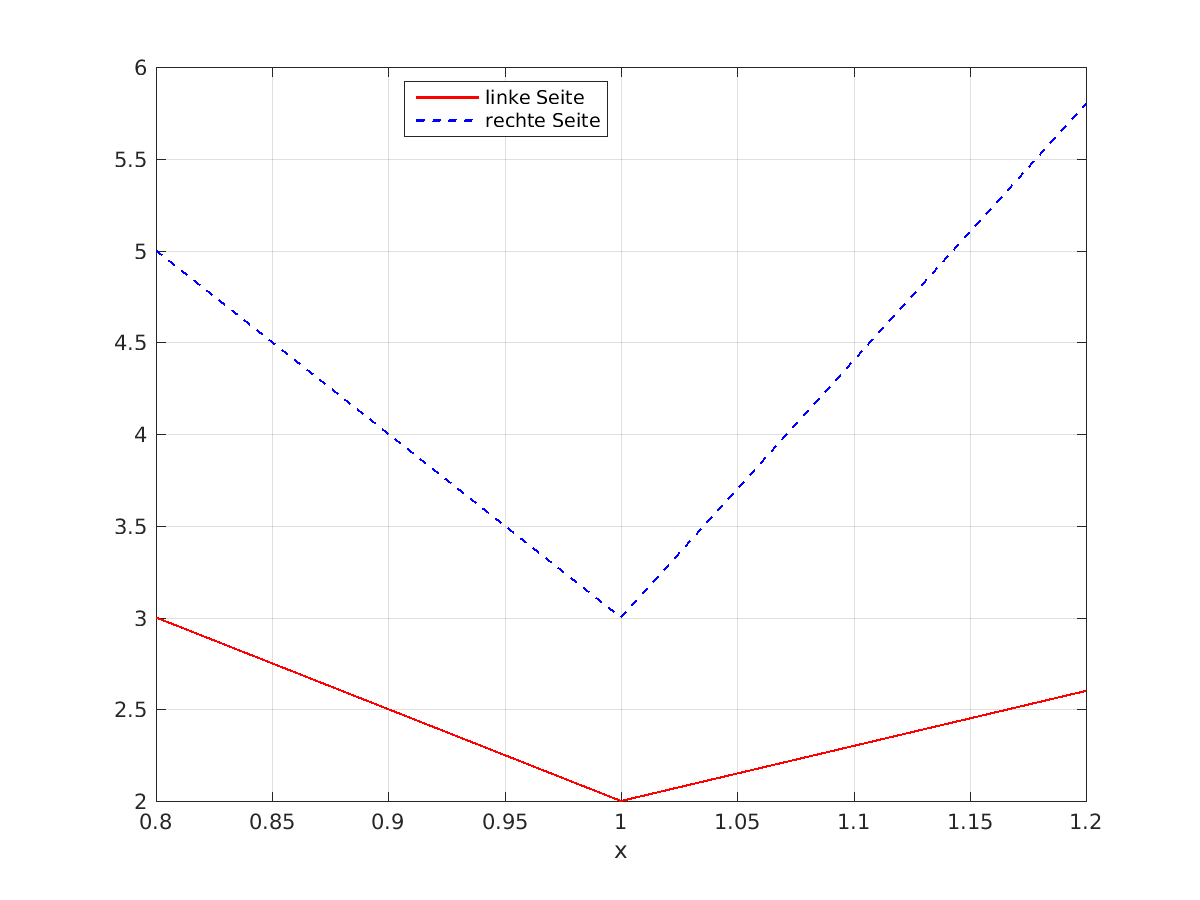
\includegraphics[width=0.8\linewidth]{Abb_zur_Ag_autogenerated_ineq_3.png} \end{center}
 
\else\relax\fi
 \end{MAufgabe}